\chapter{Results and discussion}
The implemented parser and planner makes a correct parsing and planning for
four different example inputs, which are shown in Table \ref{tab:exampleinput}. 
As seen in the second example sentence, it
also handles ambiguous sentences, i.e. handles multiple parse trees. The first
parse tree both refers to move all blocks in the world and an non-existing
block, which is the reason for the error message ''no such block''. All the
plans below assumes an initial world identical to the one shown in 
Figure \ref{fig:initworld}.\\
\begin{figure}[h!]
\centering
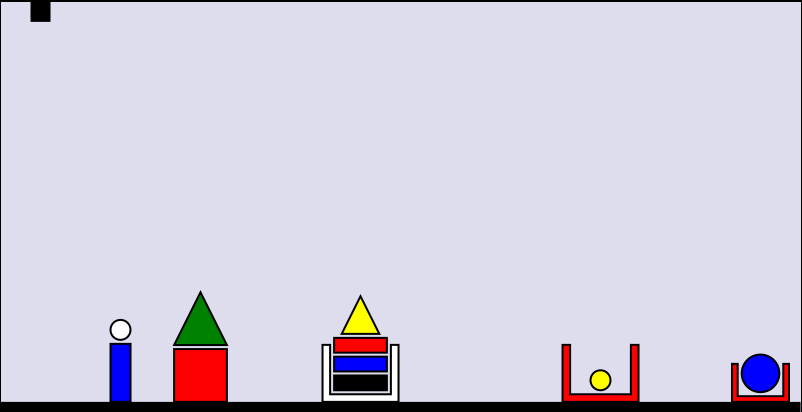
\includegraphics[scale = 0.5]{fig/1.png}
\caption{The initial world\\ $[[],[a,b],[c,d], [], [e,f,g,h,i],[],[],[j,k], [], [l,m]]$}
\label{fig:initworld}
\end{figure}\\\\
All the examples in Table \ref{tab:exampleinput} refers to a $Move$ action. An example of how a
planning is done is shown in Figure \ref{fig:moveex}. The implemented parser
and planner also handles the actions $Take$ and $Put$. Examples of these are
shown below in Table \ref{tab:put_take}. The $Put$ action assumes that there is
a holding block, in this case the world is the same as above but the robot arm 
holds the red square.
\begin{table}[p]
\centering
\begin{tabular}{| p{6cm} | p {5.8cm} | p{1.8cm} | }
\hline
\textbf{Input} & \textbf{Parse trees (concrete syntax)} & \textbf{Planning} \\ \hline
Put the blue block that is to the left of a pyramid in a medium-sized box. & ( move ( the ( thatis ( block \_ \_ blue ) ( leftof ( any ( block pyramid \_ \_ ) ) ) ) ) ( inside ( any ( block box medium \_ ) ) ) ) & 
pick 1\linebreak
drop 8\linebreak
pick 9\linebreak
drop 6\linebreak
pick 1\linebreak
drop 9\linebreak \\ \hline
Move all wide blocks inside a box on top of the red square. & ( move ( all ( block \_ wide \_ ) ) ( inside ( any ( thatis ( block box \_ \_ ) ( ontop ( the ( block square \_ red ) ) ) ) ) ) )  \newline \newline \newline
( move ( all ( thatis ( block \_ wide \_ ) ( inside ( any ( block box \_ \_ ) ) ) ) ) ( ontop ( the ( block square \_ red ) ) ) ) & "no such block" \newline \newline \newline \newline \newline
pick 4\linebreak
drop 8\linebreak
pick 2\linebreak
drop 6\linebreak
pick 4\linebreak
drop 2\linebreak
pick 4\linebreak
drop 2\linebreak
pick 4\linebreak
drop 2\linebreak \\
\hline
Put the wide blue block under the black rectangle. & ( move ( the ( block \_ wide blue ) ) ( under ( the ( block rectangle \_ black ) ) ) ) & 
pick 4\linebreak
drop 8\linebreak
pick 4\linebreak
drop 6\linebreak
pick 4\linebreak
drop 6\linebreak
pick 4\linebreak
drop 6\linebreak \\ \hline
Move all wide rectangles into a red box. & ( move ( all ( block rectangle wide \_ ) ) ( inside ( any ( block box \_ red ) ) ) ) & 
pick 4\linebreak
drop 8\linebreak
pick 7\linebreak
drop 6\linebreak
pick 4\linebreak
drop 7\linebreak
pick 4\linebreak
drop 7\linebreak
pick 4\linebreak
drop 7\linebreak \\\hline
\end{tabular}
\caption{Result of the given example sentences in the initial world}
\label{tab:exampleinput}
\end{table}
\begin{figure}[p]
\centering
\begin{subfigure}{.5\textwidth}
  \centering
  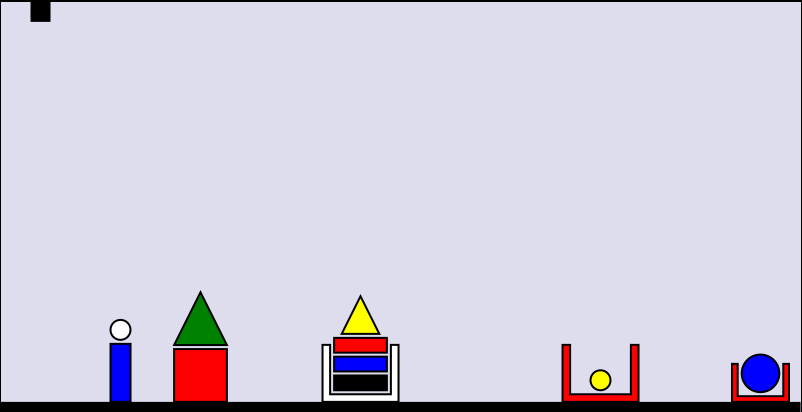
\includegraphics[width=.7\linewidth]{fig/1.png}
  \caption{Inital state}
  \label{fig:1}
\end{subfigure}%
\begin{subfigure}{.5\textwidth}
  \centering
  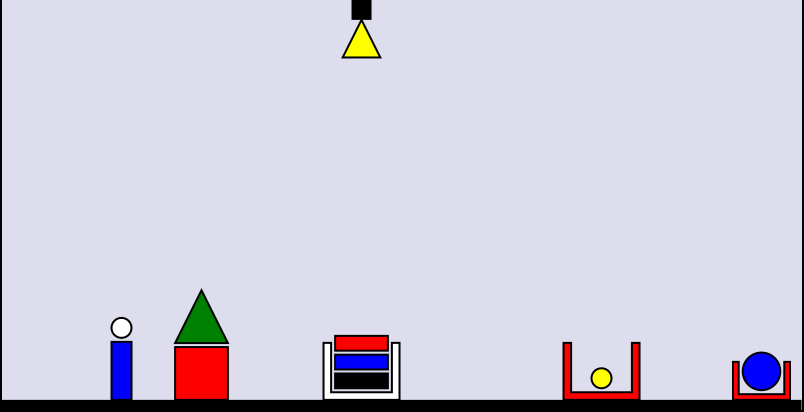
\includegraphics[width=.7\linewidth]{fig/2.png}
  \caption{Take the yellow pyramid}
  \label{fig:2}
\end{subfigure}
\begin{subfigure}{.5\textwidth}
  \centering
  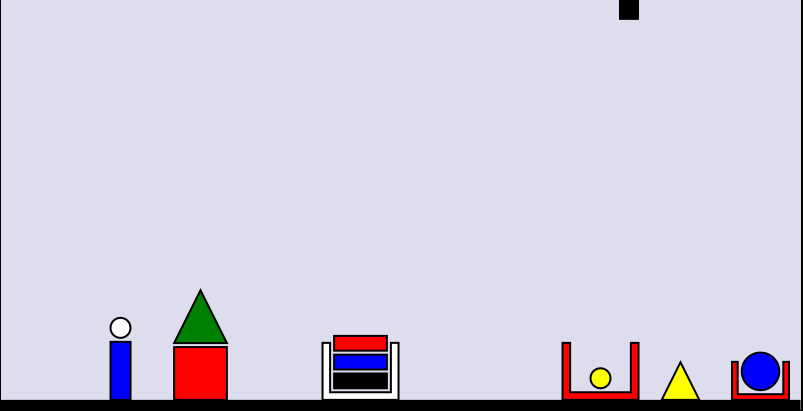
\includegraphics[width=.7\linewidth]{fig/3.png}
  \caption{Drop the yellow pyramid}
  \label{fig:3}
\end{subfigure}%
\begin{subfigure}{.5\textwidth}
  \centering
  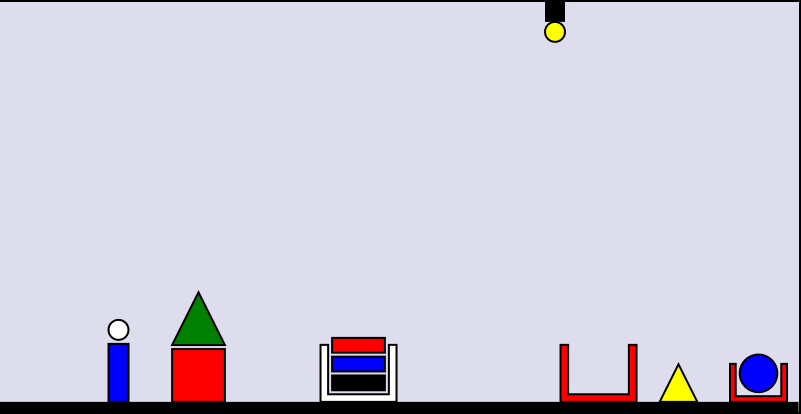
\includegraphics[width=.7\linewidth]{fig/4.png}
  \caption{Take the yellow ball}
  \label{fig:4}
\end{subfigure}
\begin{subfigure}{.5\textwidth}
  \centering
  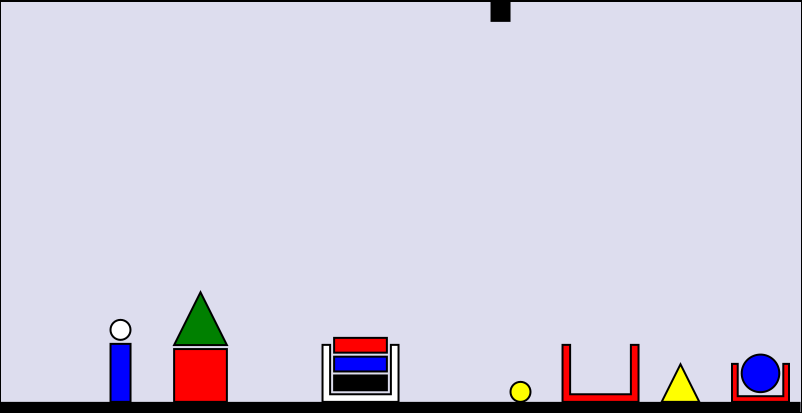
\includegraphics[width=.7\linewidth]{fig/5.png}
  \caption{Drop the yellow ball}
  \label{fig:5}
\end{subfigure}%
\begin{subfigure}{.5\textwidth}
  \centering
  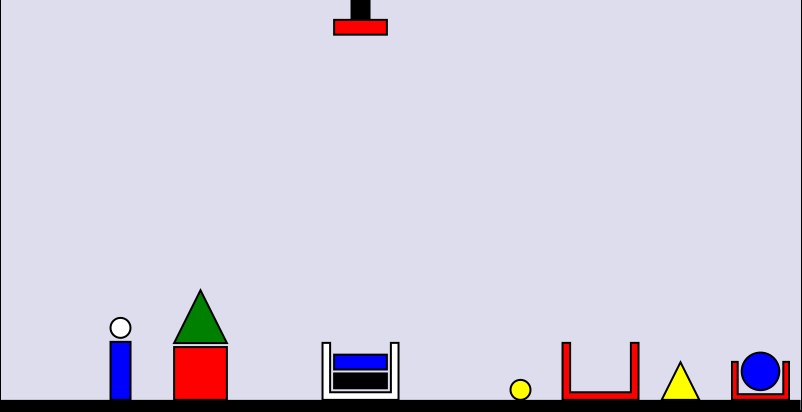
\includegraphics[width=.7\linewidth]{fig/6.png}
  \caption{Take the red rectangle}
  \label{fig:6}
\end{subfigure}
\begin{subfigure}{.5\textwidth}
  \centering
  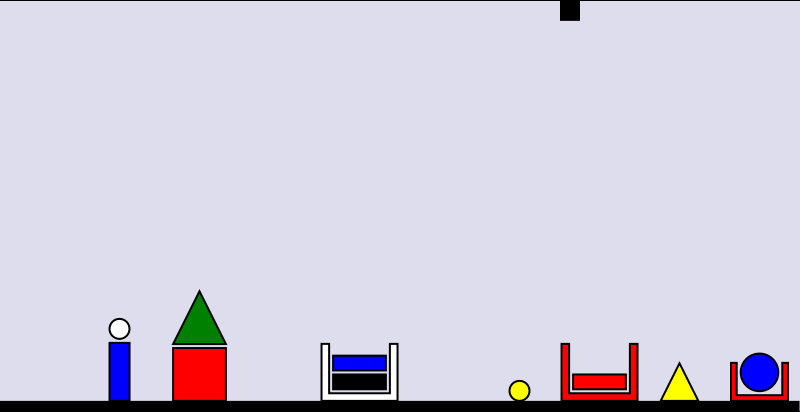
\includegraphics[width=.7\linewidth]{fig/7.png}
  \caption{Drop the red rectangle}
  \label{fig:7}
\end{subfigure}%
\begin{subfigure}{.5\textwidth}
  \centering
  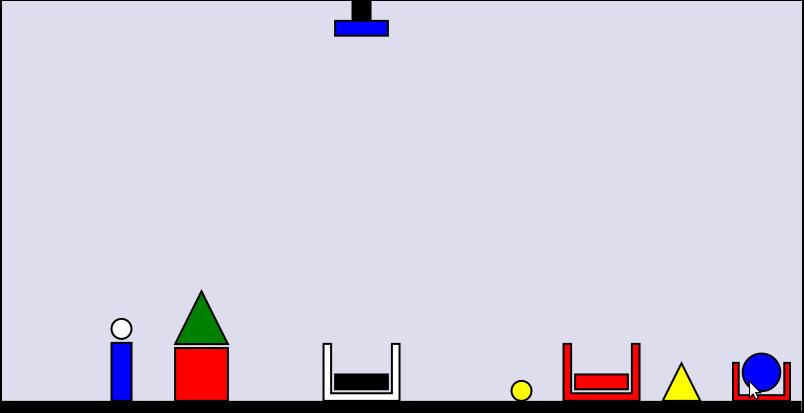
\includegraphics[width=.7\linewidth]{fig/8.png}
  \caption{Take the blue wide rectangle}
  \label{fig:8}
\end{subfigure}
\begin{subfigure}{.5\textwidth}
  \centering
  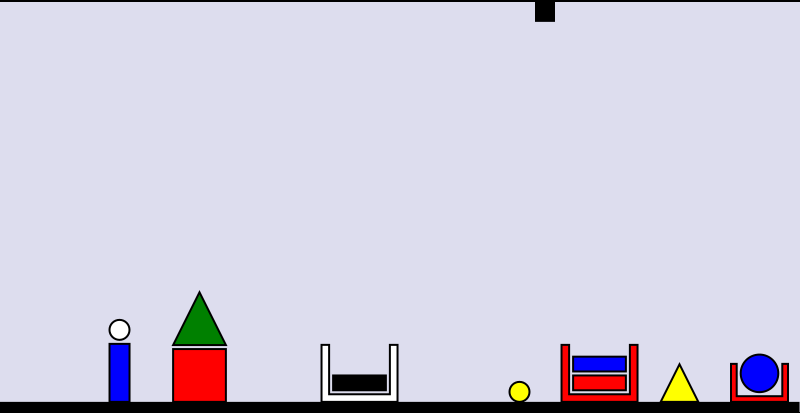
\includegraphics[width=.7\linewidth]{fig/9.png}
  \caption{Drop the blue wide rectangle}
  \label{fig:9}
\end{subfigure}%
\begin{subfigure}{.5\textwidth}
  \centering
  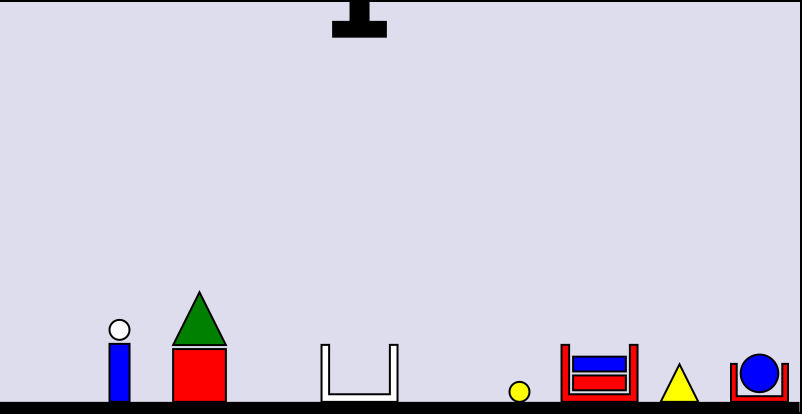
\includegraphics[width=.7\linewidth]{fig/10.png}
  \caption{Take the black rectangle}
  \label{fig:10}
\end{subfigure}
\begin{subfigure}{.5\textwidth}
  \centering
  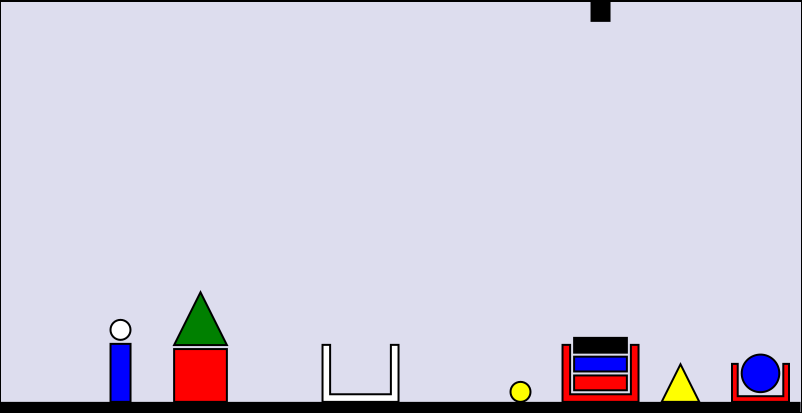
\includegraphics[width=.7\linewidth]{fig/11.png}
  \caption{Drop the black rectangle}
  \label{fig:11}
\end{subfigure}
\caption{The figure shows how the blocks are moved for the action: ''Move all wide rectangles into a red 
box.''}
\label{fig:moveex}
\end{figure}
\begin{table}[h!]
\centering
\begin{tabular}{| p{6cm} | p {5.8cm} | p{1.8cm} | }
\hline
\textbf{Input} & \textbf{Parse trees (concrete syntax)} & \textbf{Planning} \\ \hline
Take the red square! & 	(take (the (block square \_ red ) ) ) & 
pick 2\linebreak
drop 8\linebreak
pick 2\linebreak\\ \hline
Put it on the floor & ( put ( ontop floor) ) & drop 6\linebreak \\ \hline
\end{tabular}
\caption{Result of actions $Take$ and $Put$ (when holding the block from the $Take$ action}
\label{tab:put_take}
\end{table}\\\\
Of course there are several sentences which are not handled by the parser and the
planner. An example of a such sentence is "Move all blocks inside a box on top
of the red square." which results in a timeout due to our translation of the
command. The parser returns a list of all blocks that is inside of a box, to be
moved. This is impossible to perform in the initial world since there are two
boxes with a ball inside and balls can never be put on each other. Then the
planner will not find a solution, which results in a timeout.\\\\
The planner does not print what it does, such as ''I move the topmost block
from stack X to stack Y''. The planning is just shown visually and in form of
pick and drop instructions. \\\\
The planner will not try to optimize the time it takes to perform the
instructions, i.e. it might not drop blocks at the closest available stack.
This does not affect the number of instructions, which we try to optimize.
Also, the planner will not try to restore blocks to their initial positions if
it has move them to reach another block or position. 
\\\\
If the sentence is ambiguous, the parser will return multiple parse tree but
the planner will only choose the first valid parse tree. In the example
sentence 2, the first parse tree is treated as invalid. 
\\\\
Another thing worth mention is that the parser does not make any difference of
$any$, $the$ and $all$. It always returns a list of all possibilities to the
planner. The planner does not handle those differently either, so the result will be 
the same which in practice means that some sentences will not act as expected. E.g. 
take the sentence ''Put a ball in the box''. If there are multiple balls in the world, 
this will give a timeout since the planner will try to move all balls into the box and 
balls are not allowed to be on top of each other. Also, ''the box'' may refer to 
multiple boxes but only the first one in the list will be chosen. The correct behavior of 
the parser and the planner would be to chose one ball, which is easiest to move and therefore 
best according to the heuristic function, and move it into the box, specified 
by the user. 
\section{Discussion}
A well-known problem when handling natural languages is that there are many ways of interpreting
things which easily makes a sentence ambiguous. We also noticed that it was
hard to cover all cases that could occur in the parser and depending on which
input we got it was possible to pattern match on power sets of possible inputs,
which maked the code increase rapidly. \\\\
Another difficulty in the beginning was that the syntax tree that was given
from the parser was a concrete syntax tree and we wanted an abstract syntax
tree to be able to pattern match on the different parts. This was solved when
we found a library which could convert between GF grammar as concrete and
abstract syntax. \\\\
We did a lot of tweaking with the heuristic function and notice how instable it
was. There might be cases that we miss and there are a lot of ways of making a
heuristic function.
\\\\
Our choice was to implement a planning algorithm by graph traversal, by
implementing A*. Another possibility would have been to use for example First-Order
Logic instead but the group had prior knowledge of graph traversal and with the time 
given it seemed most reasonable to come up with an effecient planner using our prior knowledge. 
\\\\
We had many discussions about have to treat $any$, $the$ and $all$ in the
parser and the difference of these. This resulted in that they were treated in
the same way which is not correct. If we would had more time, a possible solution 
of how to treat these could be the following: 
\begin{itemize}
\item if $any$, the planner could treat the possibilities as different parse trees and choose the best one. 
\item if $the$, and there is more than one possibility the system should let the user specify which one was meant. 
\item if $all$, all possibilities should be returned to the planner
\end{itemize}
